\section{The VSI with realistic  protoplanetary disk cooling}\label{application} 
To this point we have treated the cooling time, $\beta$, as a free
parameter that, moreover, is independent of height.  
To understand the applicability of the VSI to PPDs, we now consider
$\beta$ values that are consistent with PPD models. 
Section \ref{cooling_model}  develops our PPD cooling law, which
depends on disk radius, disk height and perturbation wavelength. 
We compare these PPD $\beta$ values to $\beta_{\rm crit}$ in
\S\ref{bcritPPD}.  While this comparison is instructive, it is not
complete since $\beta_{\rm crit}$ was derived assuming a vertically
constant $\beta$.  Thus in \S\ref{vsi_mmsn_grow} we analyze the linear
growth of VSI with our PPD $\beta$ values. 

% As an application of our linear models, we estimate where in a
% PPD do the thermodynamic conditions allow the VSI to
% operate. We first model the cooling time $t_c$ based on realistic
% disk properties, which yields a non-uniform dimensionless cooling
% time $\beta(r,z;\khat)$. We then compare this to the critical cooling time
% $\beta_\mathrm{crit}$ derived above. Finally, we explicitly compute 
% linear growth rates numerically, using $\beta(r,z;\khat)$, to
% characterize growth times expected in a typical PPD.   

%linearized RHS of Eq. \ref{real_energy} by a thermal
%relaxation time $t_c$.
% For a realistic disk one might consider an energy equation
% with radiative cooling, 
% \begin{align}\label{real_energy}
%   % \rho T \frac{DS}{Dt} = - \left(\nabla\cdot\bm{F} - Q_+\right), 
%   \frac{\p P}{\p t} + \bm{v}\cdot\nabla P +\gamma P \nabla\cdot\bm{v} = - \frac{P}{\rho T
%     C_v}\left(\nabla\cdot\bm{F} - Q_+\right), 
% \end{align}
% where $C_v$ is the heat capacity at constant
% volume, 
% $\bm{F}$ is the radiative flux and $Q_+$ is a heating
% term to permit an equilibrium solution. 
% One should now model in detail each of the terms on the RHS of
% Eq. \ref{real_energy}, linearize them, then solve 
% the resulting linear eigenvalue problem. This is beyond 
% the scope of the present work.

\subsection{Cooling model} \label{cooling_model}

\subsubsection{Radiative diffusion and Newtonian cooling}
The thermal relaxation of a perturbation depends on the relative sizes of the perturbation's 
lengthscale, $l$, and the photon mean-free-path,
\begin{align}\label{lrad}
  l_\mathrm{rad} \equiv \frac{1}{\kappa_d\rho} 
\end{align}
where $\kappa_d$ is the opacity, specifically the dust opacity appropriate for cold PPDs. 

In the optically thick limit, $l\gg l_\mathrm{rad}$, radiative diffusion smooths out thermal perturbations.
In this regime, the linearized cooling function is

\begin{align}\label{diff_cool_proper}
  \delta \Lambda_\mathrm{diff} = \frac{P}{\rho T C_v} \nabla\cdot\left(k_\mathrm{rad}\nabla\delta
    T\right),  
\end{align}
where $k_\mathrm{rad}$ is the radiative conduction coefficient defined
below, and $C_v$ is the specific heat capacity at constant volume. 

Since the VSI is characterized by vertically-elongated,
radially-narrow disturbances, we retain only the radial derivatives of
the perturbations in Eq. \ref{diff_cool_proper}. 
Thus, in the radially local approximation, we have
\begin{align}\label{diff_cool_approx}
  % \frac{P}{\rho T C_v} \nabla\cdot\left(k_\mathrm{rad}\nabla\delta
  %  T\right) &
  \delta\Lambda_\mathrm{diff} \simeq %-\frac{k_\mathrm{rad}}{\rho
  % C_v}k_x^2P\left(\frac{\delta T}{T}\right)%\notag\\
  % \equiv 
  %-\eta k_x^2 \left(\delta P - \frac{P}{\rho}\delta\rho\right) =
  -\eta k_x^2 P \frac{\delta T}{T}, %=
  %-\frac{P}{t_\mathrm{diff}}\frac{\delta T}{T},
  %\frac{P}{t_\mathrm{diff}}\left(\frac{delta T}{T}\right), 
\end{align}
where the radiative diffusion coefficient is
\begin{align}\label{eta_def}
  \eta \equiv {k_\mathrm{rad} \over \rho C_v} = \frac{16\sigma_s T^3}{3\kappa_d\rho^2 C_v}, 
\end{align}
and $\sigma_s$ is the Stefan-Boltzmann constant. 
The thermal relaxation  timescale (defined in Eq. \ref{thermal_relax}) 
for radiative diffusion is thus 
\begin{align}\label{tc_diff_cool} 
  t_\mathrm{diff} = \frac{1}{\eta k_x^2}.%\equiv \frac{\OmK^{-1}}{\hat{\eta}\khat^2}, 
\end{align}

In the optically thin regime, $l\ll 
l_\mathrm{rad}$, thermal relaxation operates by `Newtonian cooling'.
The cooling time is independent of $l$ and 
inversely proportional to the opacity, $t_\mathrm{thin} \propto 1/\kappa_d$. 
Specifically 
\begin{align}
  t_\mathrm{thin} = \frac{l_\mathrm{rad}^2}{3\eta},
\end{align}
and $t_\mathrm{thin}$ does not depend on $\rho$ (because our adopted
$\kappa_d$ depends on $T$ only, see below). 

Our general cooling time for all perturbations,
\begin{align}\label{tc_def}
  t_c &\equiv t_\mathrm{thin} + t _\mathrm{diff},%=
  % \frac{l_\mathrm{rad}^2}{3\eta} + \frac{1}{\eta k_x^2},  
\end{align}
is a simple prescription to smoothly match the optically thick and thin limits.

\subsubsection{PPD cooling times}\label{toy_relax}
In a vertically isothermal disk with surface density $\Sigma = \rho_0\sqrt{2\pi}H$, 
the dimensionless thermal
relaxation time $\beta$ becomes 
\begin{align}\label{real_beta}
  \beta(r,z;\khat) \equiv t_c\OmK =
  % \frac{1}{\hat{\eta}}\left[\frac{l_\mathrm{rad}^2}{3H^2}
  %   + \frac{\hat{\rho}^2(z)}{2\pi\khat^2}\right]  \simeq
  \frac{\Sigma^2\OmK}{\eta\rho^2}\left[\frac{1}{3\kappa_d^2\Sigma^2} 
    + \frac{\hat{\rho}^2(z)}{2\pi \khat^2}\right].
\end{align}
where $\hat{\rho} = \rho/\rho_0$.  The first and second terms in
square brackets represent the optically thin and thick cooling
regimes, respectively. 

We adopt the Minimum Mass Solar Nebula
(MMSN) disk model of \cite{chiang10} which specifies
% \emph{note that the normalizations are suppressed b/c I can't see where we used them.  We should only add back in if we decide to use them.}
\begin{subequations}
\begin{align}
\label{mmsn_sigma}
  \Sigma &= 2200 %\hat{\Sigma}\left(\frac{r}{\mathrm{AU}}\right)^{-3/2}
 r_\mathrm{AU}^{-3/2} \mathrm{g}\,\mathrm{cm}^{-2},  \\
 T &= 120%\hat{T}\left(\frac{r}{\mathrm{AU}}\right)
  r_\mathrm{AU}^{-3/7} \mathrm{K}, \label{mmsn_temp}  
\end{align}\end{subequations}
with $r_\mathrm{AU}\equiv r/\mathrm{AU}$. This model has $q = -3/7$,
$p = -39/14$ and $h  = 0.022 r_\mathrm{AU}^{2/7}$, using $\mu = 2.33$
and the above relation between $\Sigma$ and $\rho_0 \propto r^p$.   

For the dust opacity we adopt the \citet{bell94} law with $\kappa_d
\propto T^2$, giving 
\begin{align}
 \kappa_d %&= 2 \hat{\kappa}_d \left(\frac{T}{100\mathrm{K}}\right)^2 \mathrm{cm}^2\,\mathrm{g}^{-1}
    =
   2.88\hat{\kappa}_d r_\mathrm{AU}^{-6/7}\mathrm{cm}^2\,\mathrm{g}^{-1},   
\end{align}
where the opacity normalization factor, $\hat{\kappa}_d$, scales with
the ratio of small dust to gas;  $\hat{\kappa}_d = 1$ is our fiducial
case. 

%and summarized in
%Appendix \ref{mmsn} (where an opacity model is also chosen). Defining
%$r_\mathrm{AU}\equiv r/\mathrm{AU}$, we find Eq. \ref{real_beta}
%becomes 
% \begin{align}\label{beta_mmsn}
%   \beta(r, z; \khat) =
%   &\frac{4.4\times10^5}{\mu(\gamma-1)}\left(\frac{\hat{\kappa}_d\hat{\Sigma}^2}{\hat{T}}\right)r_\mathrm{AU}^{-57/14}\notag\\ 
%   &\times\left[\frac{8.3\times10^{-9}}{\hat{\kappa}_d^2\hat{T}^4\hat{\Sigma}^2}r_\mathrm{AU}^{33/7}+\frac{\hat{\rho}^2(z)}{2\pi\khat^2}\right].         
% \end{align} 
% We shall consider the case $\gamma=1.4$, $\mu=2.33$ with scalings
% $\hat{\Sigma}=\hat{T}=1$, and refer to this as the Minimum Mass Solar 
% Nebulae (MMSN) where $\beta=\beta_\mathrm{MMSN}$, \\
% \emph{I would keep $\kappa$ scaling in this eqn, since it's used in plots.  Then just say  that $\kappa_d = 1$ is fiducial case. }

For this disk and opacity model, the cooling time becomes
\begin{align}\label{beta_mmsn_simp}
  \beta(r,z;\khat)\notag = &3.9\times10^{-3}\hat{\kappa}_d^{-1}
  r_\mathrm{AU}^{9/14}
  \notag\\ &\times \left[1 +
    1.9\times10^7\hat{\kappa}_d^{2}\hat{\rho}^2(z)r_\mathrm{AU}^{-33/7}\khat^{-2}\right]. 
\end{align}
Perturbations are in the optically thin regime for
\begin{align}
  \khat\gtrsim 2.5\times10^3\hat{\kappa}_d\hat{\rho}(z)r_\mathrm{AU}^{-33/14}.  
\end{align}
In the inner disk, e.g. $r_\mathrm{AU}\sim 1$, only
extremely small-scale perturabtions are in the optically-thin
regime near the midplane. However, in the outer disk, e.g. $r_\mathrm{AU}\sim 10$, 
 more moderate wavenumbers $\khat\gtrsim 10$ experience optically-thin cooling.

\begin{figure}
  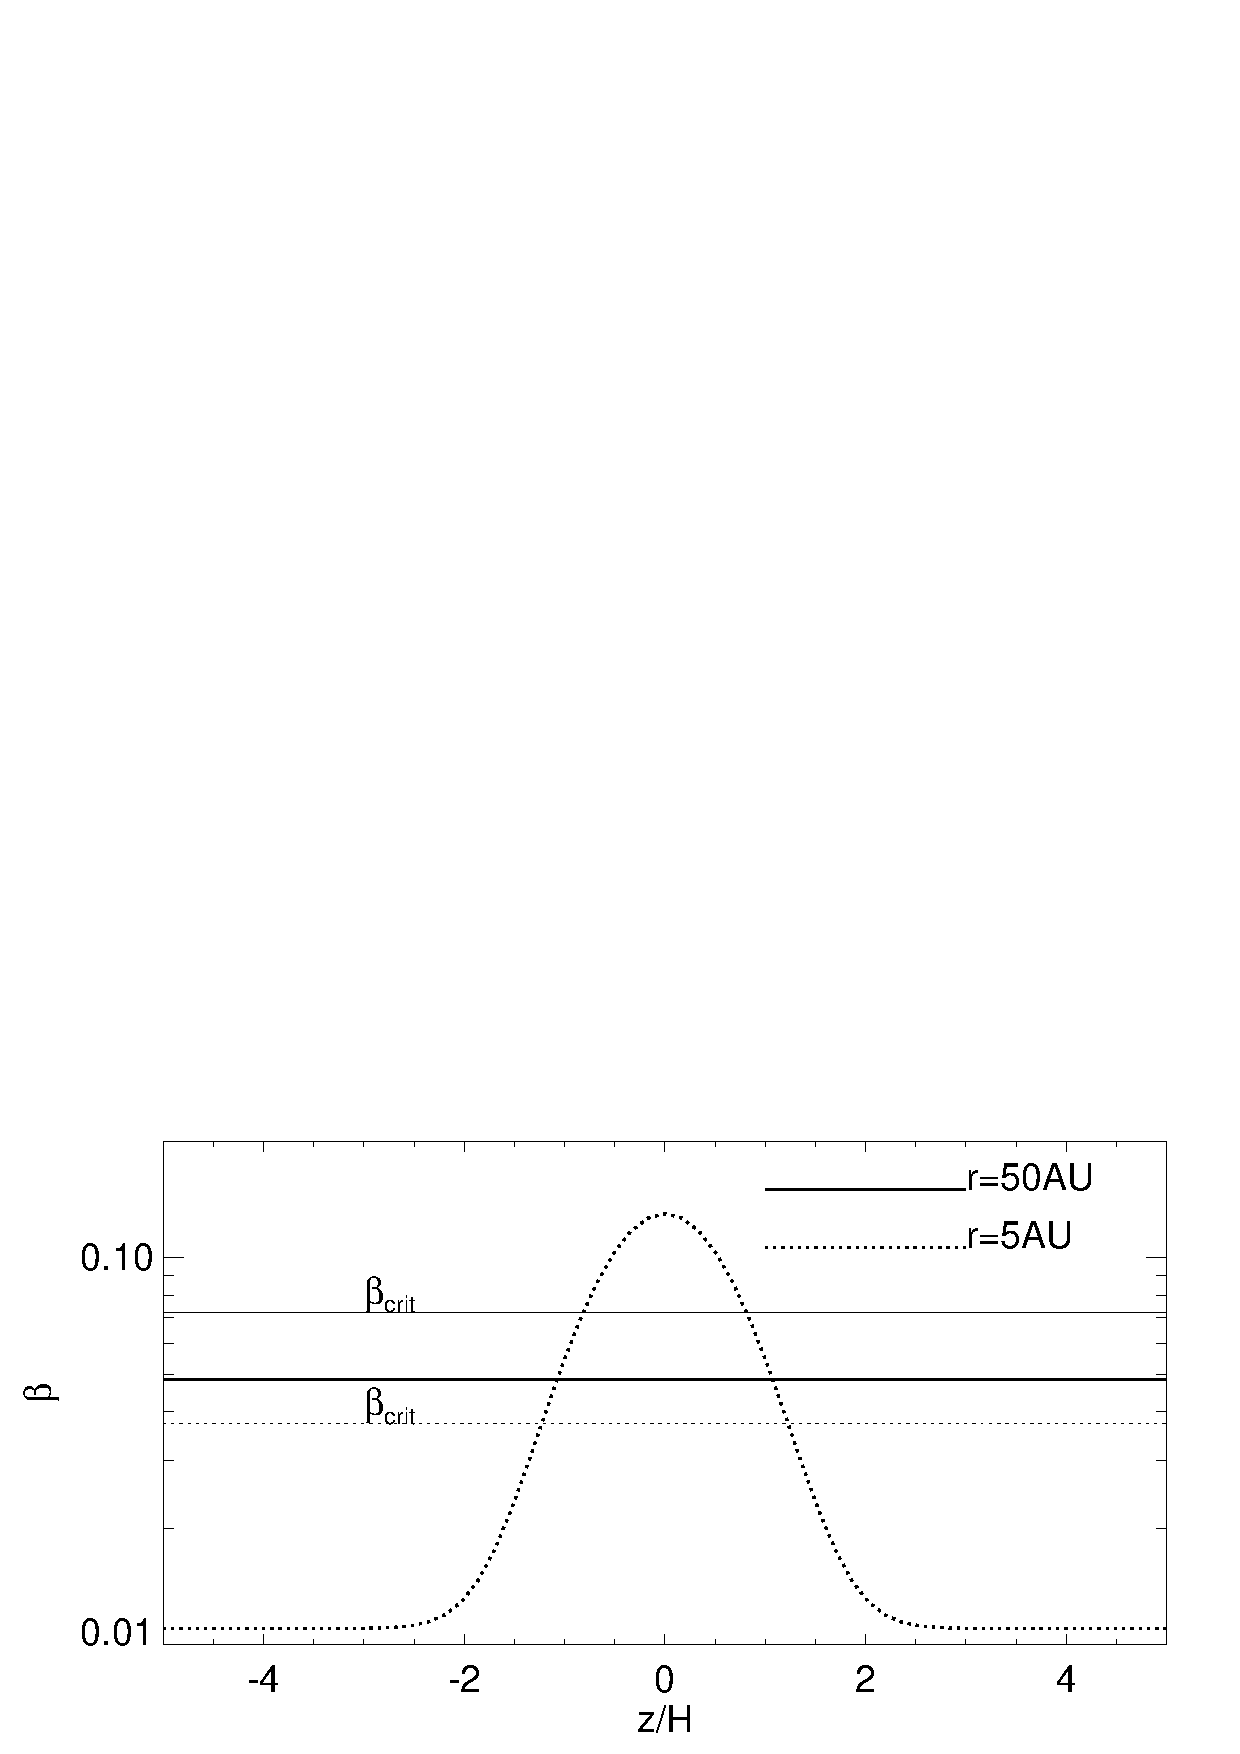
\includegraphics[width=\linewidth,clip=true,trim=0cm 0cm 0cm
  0cm]{figures/beta_compare}
  \caption{Thermal relaxation timescales in the fiducial MMSN at $r=50$AU
    and $r=5$AU for $\khat=30$ (solid lines). The
    corresponding horizontal dashed lines are the critical thermal
    relaxation timescales derived in linear theory. 
    \label{beta_compare}}
\end{figure}


\subsection{$\beta$ vs.\ $\beta_\mathrm{crit}$ in PPDs}\label{bcritPPD} 
The simplest way to estimate whether the VSI can operate at a given radius in a PPD is to 
compare the cooling time (Eq. \ref{beta_mmsn_simp}) to 
its critical value (Eq. \ref{iso_vsi_cond}), evaluated for the MMSN as    
\begin{align}\label{bcrit_mmsn}
  % \beta_\mathrm{crit} = \frac{1.44\times10^{-2}}{(\gamma
  % -1)}\left(\frac{\hat{T}}{\mu}\right)^{1/2}r_\mathrm{AU}^{2/7}. 
  \beta_\mathrm{crit} = 0.024r_\mathrm{AU}^{2/7}. 
\end{align}

This comparison is strictly valid only for optically thin cooling
which is independent of height, as assumed in the derivation of
$\beta_\mathrm{crit}$.  This condition typically holds in the outer
disk.   Fig. \ref{beta_compare} shows that a  $\khat=30$ perturbation
at 50AU has vertically constant $\beta$. Furthermore, since $\beta <
\beta_\mathrm{crit}$, the disturbance would be unstable. 
 
For optically thick cooling, $\beta$ varies with height, complicating
the comparison with $\beta_\mathrm{crit}$.    
At 5AU, Fig. \ref{beta_compare} shows that cooling times are long in
the midplane with $\beta > \beta_\mathrm{crit}$. 
However, since $\beta < \beta_\mathrm{crit}$ away from the midplane,
we require the analysis of \S\ref{vsi_mmsn_grow} to determine if the
VSI can grow.  (That calculation will show that growth is stongly
suppressed for this case.)  We proceed with the awareness that
optically thick regions in the inner disk are a complication, but that
we can reasonably expect VSI growth if $\beta < \beta_\mathrm{crit}$
at all heights. 


%Fig. \ref{beta_compare} show examples of $\beta$ in the fiducial disk
%at $r_\mathrm{AU}=5$ and $r_\mathrm{AU}=50$ for a perturbation wavenumber $\khat=30$.  
%At $r_\mathrm{AU}=50$, the disturbance is in the optically-thin regime,  
%$\beta$ is vertically uniform, as assumed for our analysis, and $\beta
%< \beta_\mathrm{crit}\, \forall z$. Accordingly we expect, and find, the VSI
%operates.     
%
%On the other hand, at $r_\mathrm{AU}=5$, the perturbation is in the optically
%thick (thin) regime near (away from) the midplane. In this case,
%$\beta < \beta_\mathrm{crit}$ for $|z|\gtrsim1.25H$. Our analytic 
%criteria is not valid for vertically non-uniform $\beta$ so we must
%turn to numerical solutions of the linear problem. We do this in
%\S\ref{vsi_mmsn_grow}. % and find the VSI also operates in this case, but
%% with significantly reduced efficiency. 
%
%%, as
%% described below.  


\begin{figure*}
  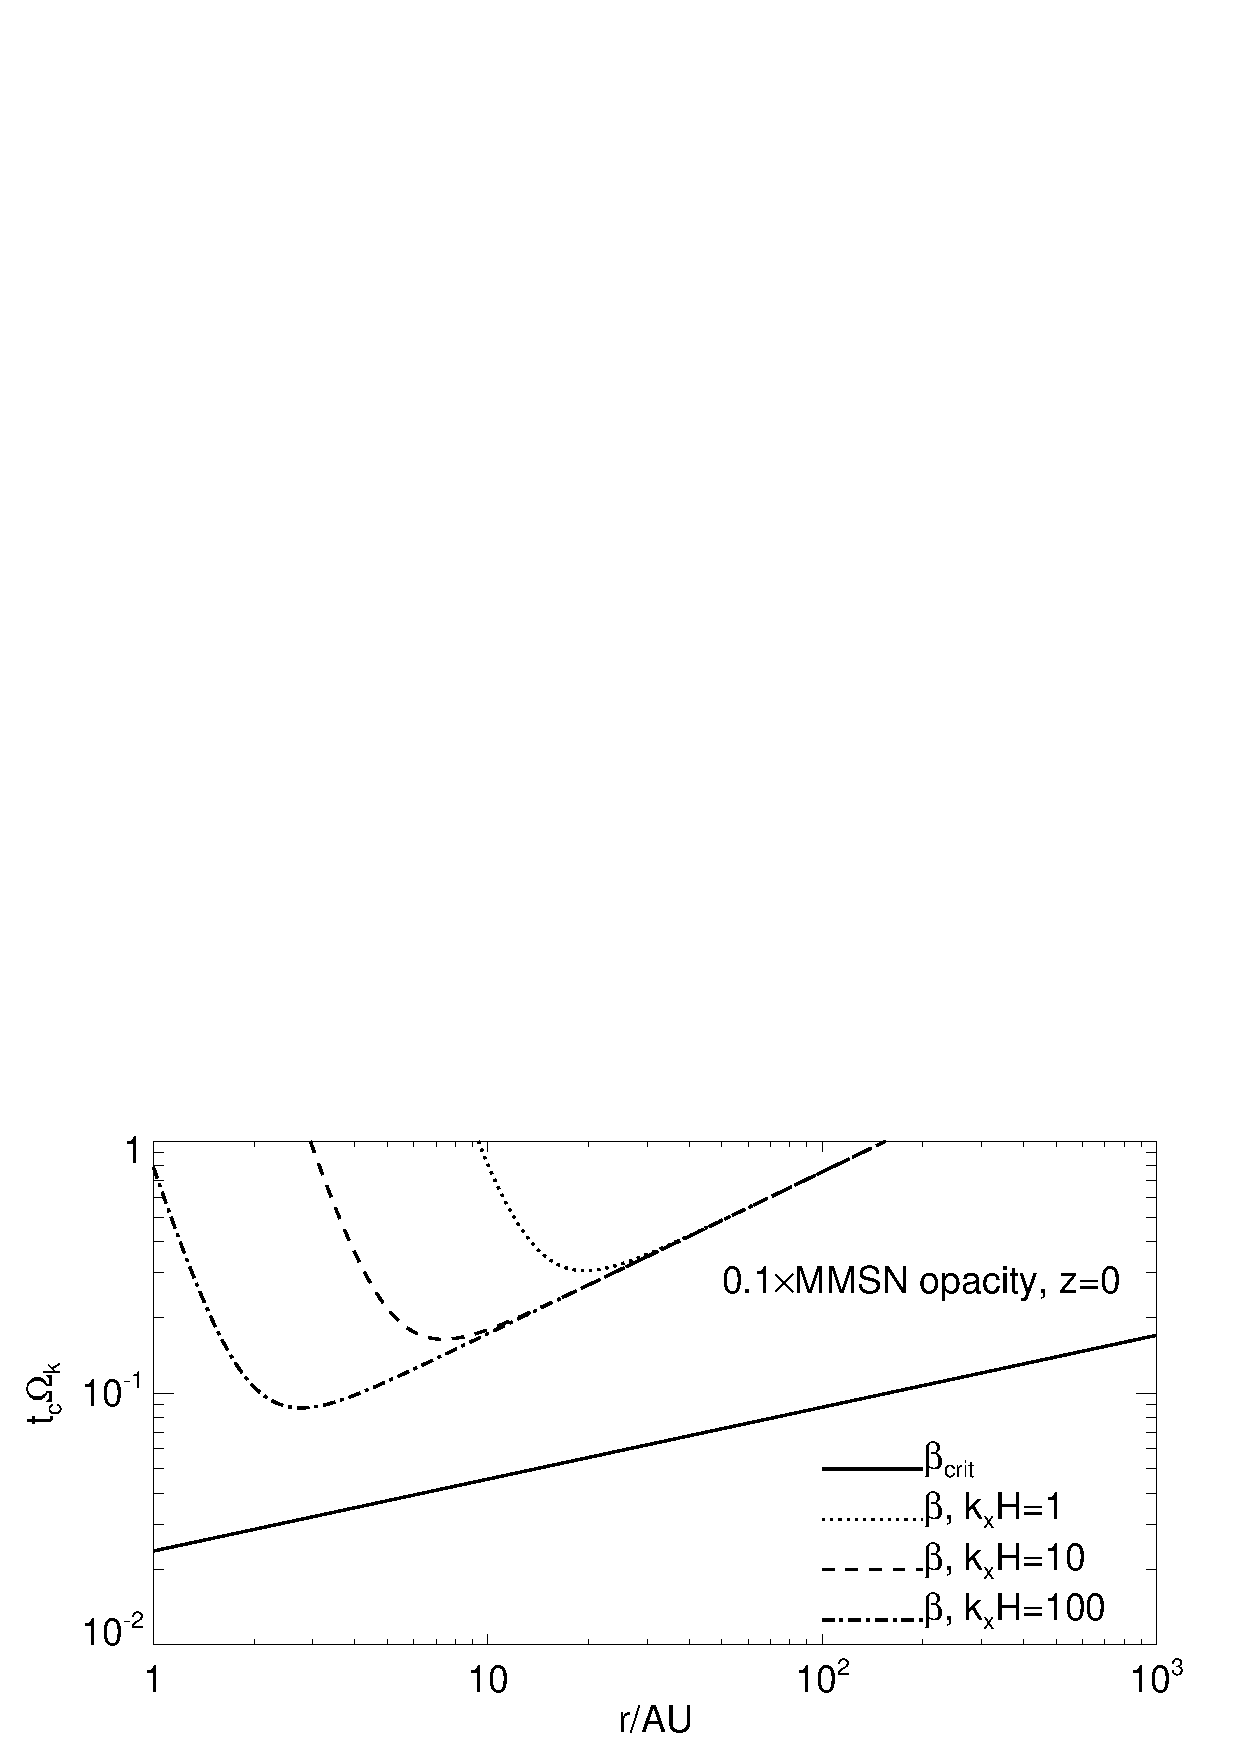
\includegraphics[scale=.47,clip=true,trim=0cm 1.8cm 0cm
  0cm]{figures/bcrit_mmsn_kap0d1_z0}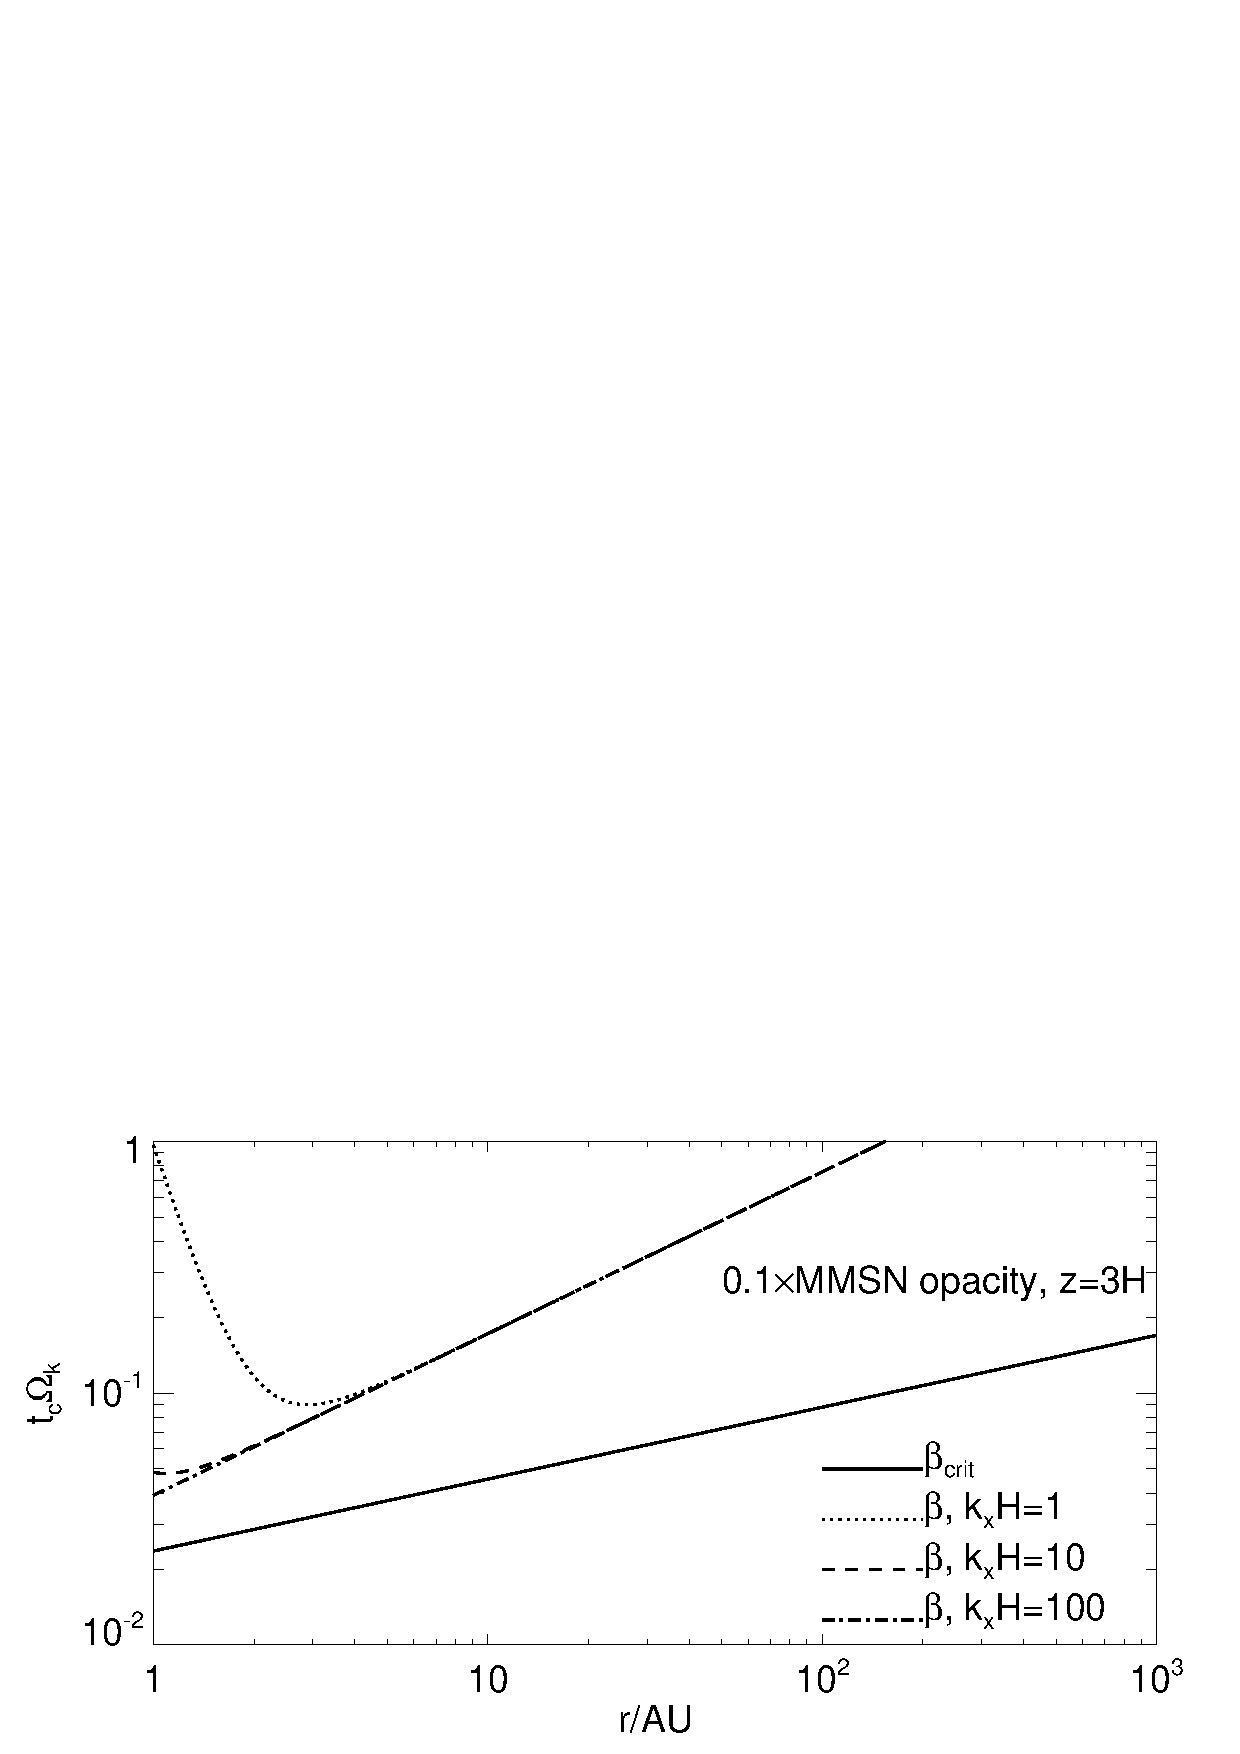
\includegraphics[scale=.47,clip=true,trim=2.5cm 1.8cm 0cm
  0cm]{figures/bcrit_mmsn_kap0d1_z3}\\ 
  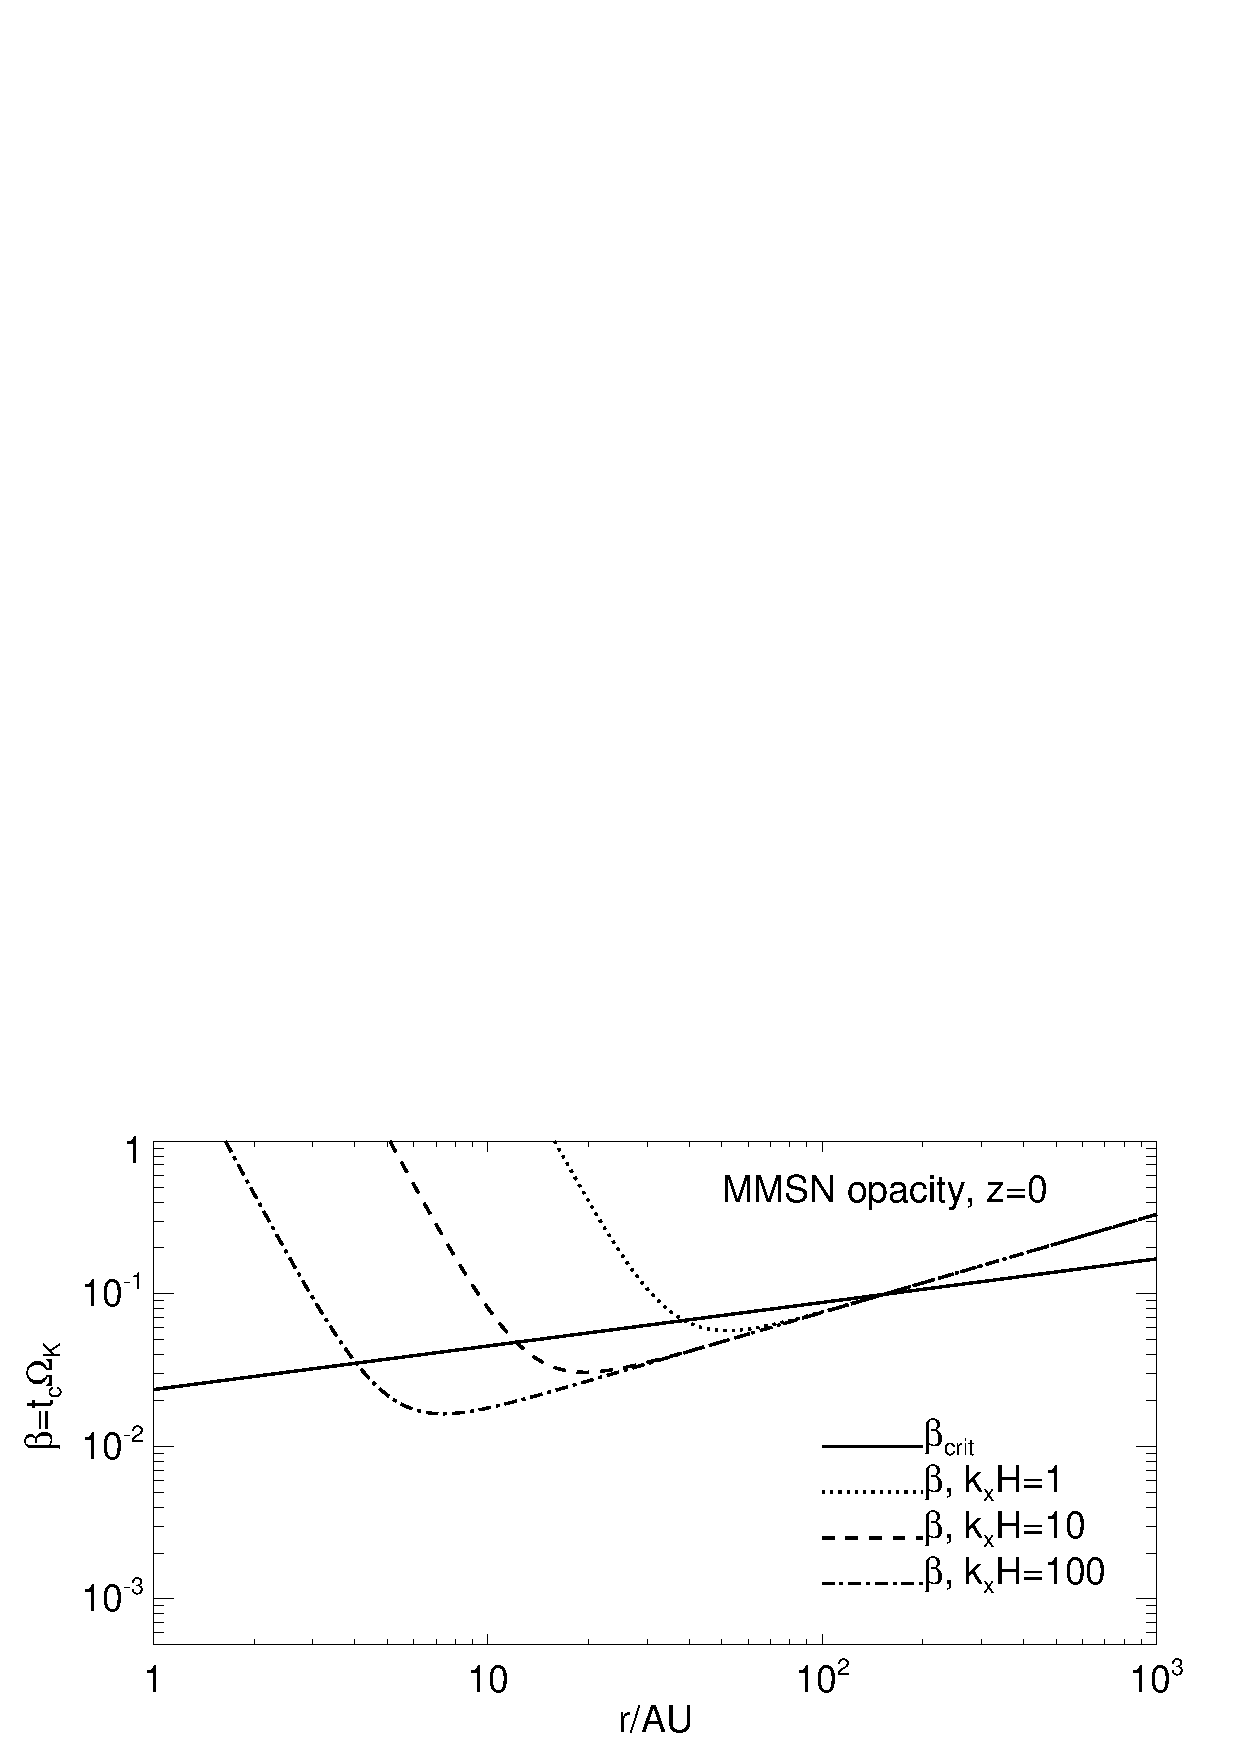
\includegraphics[scale=.47,clip=true,trim=0cm 1.8cm 0cm
  1cm]{figures/bcrit_mmsn_kap1_z0}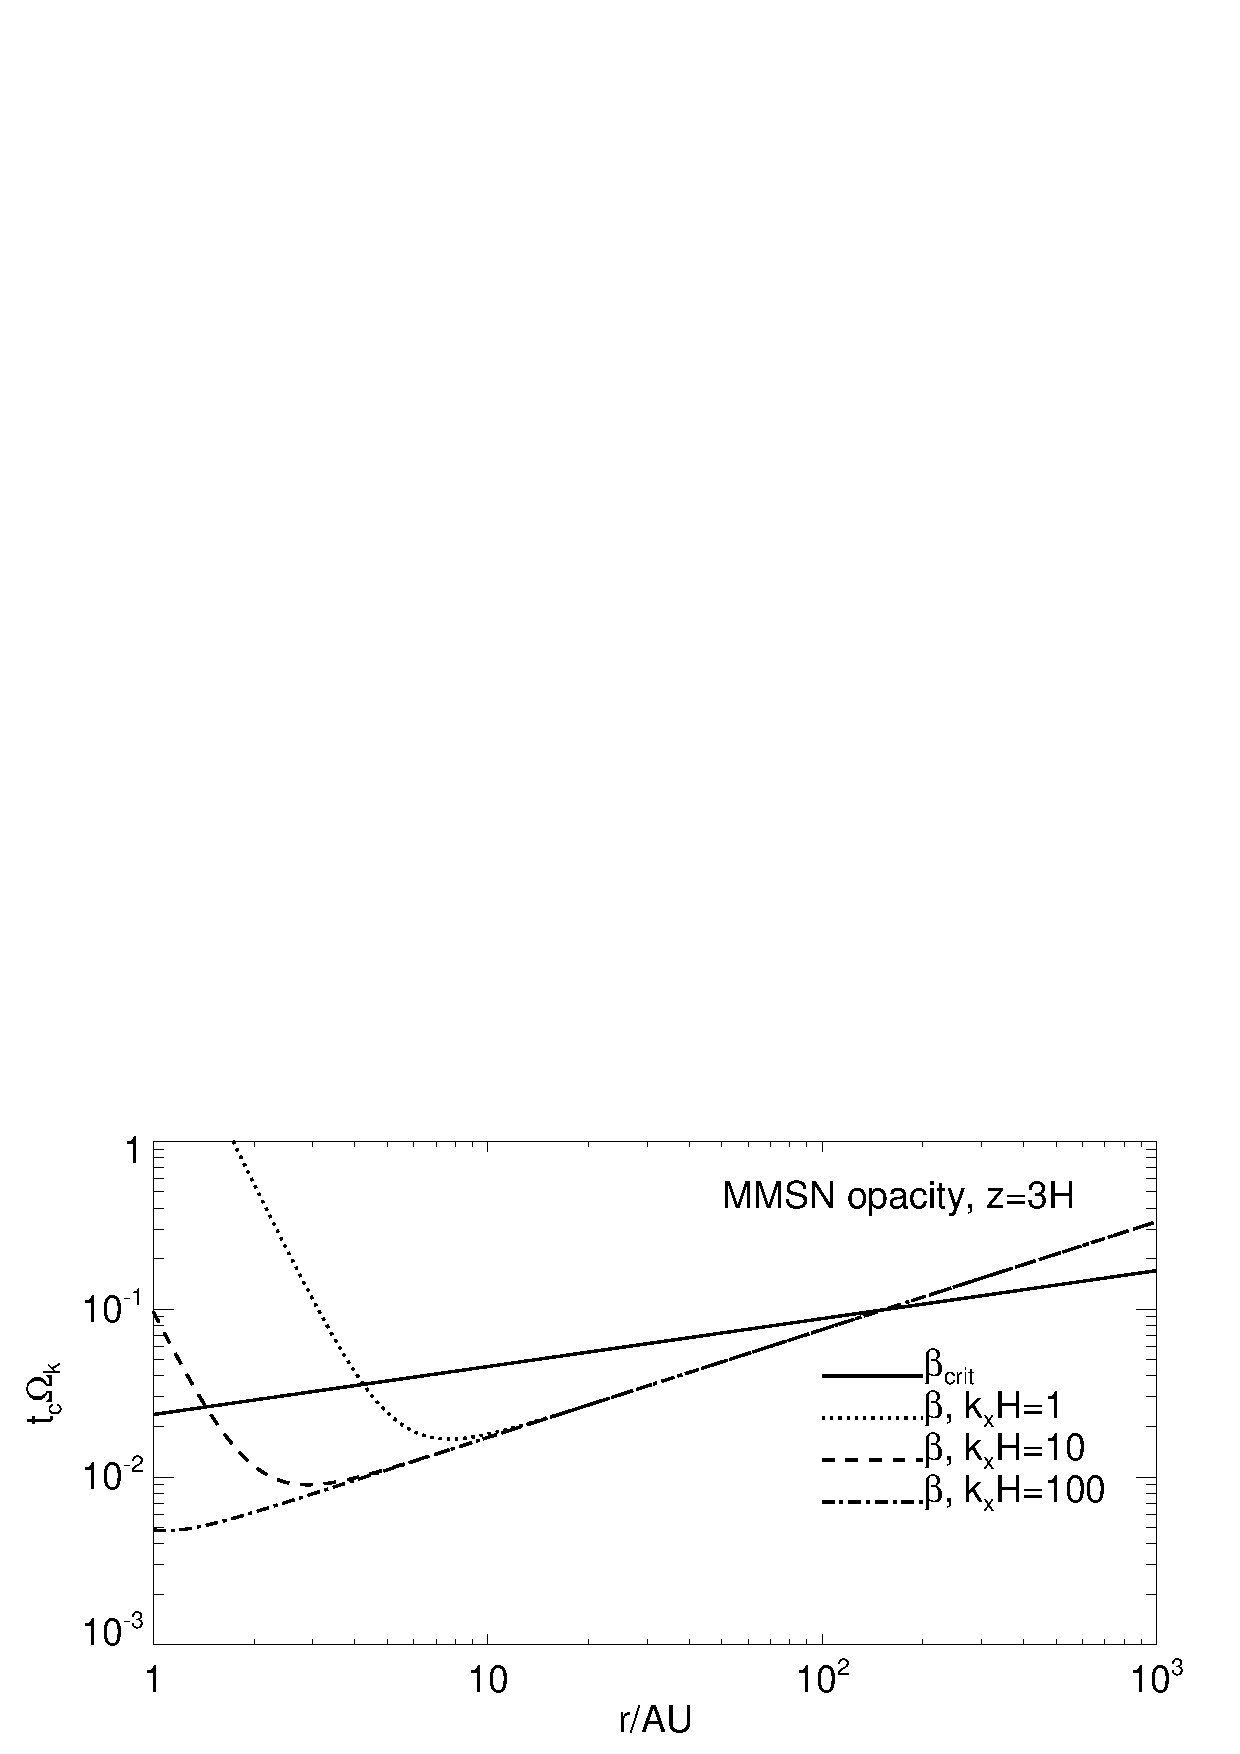
\includegraphics[scale=.47,clip=true,trim=2.5cm
  1.8cm 0cm 1cm]{figures/bcrit_mmsn_kap1_z3}\\
  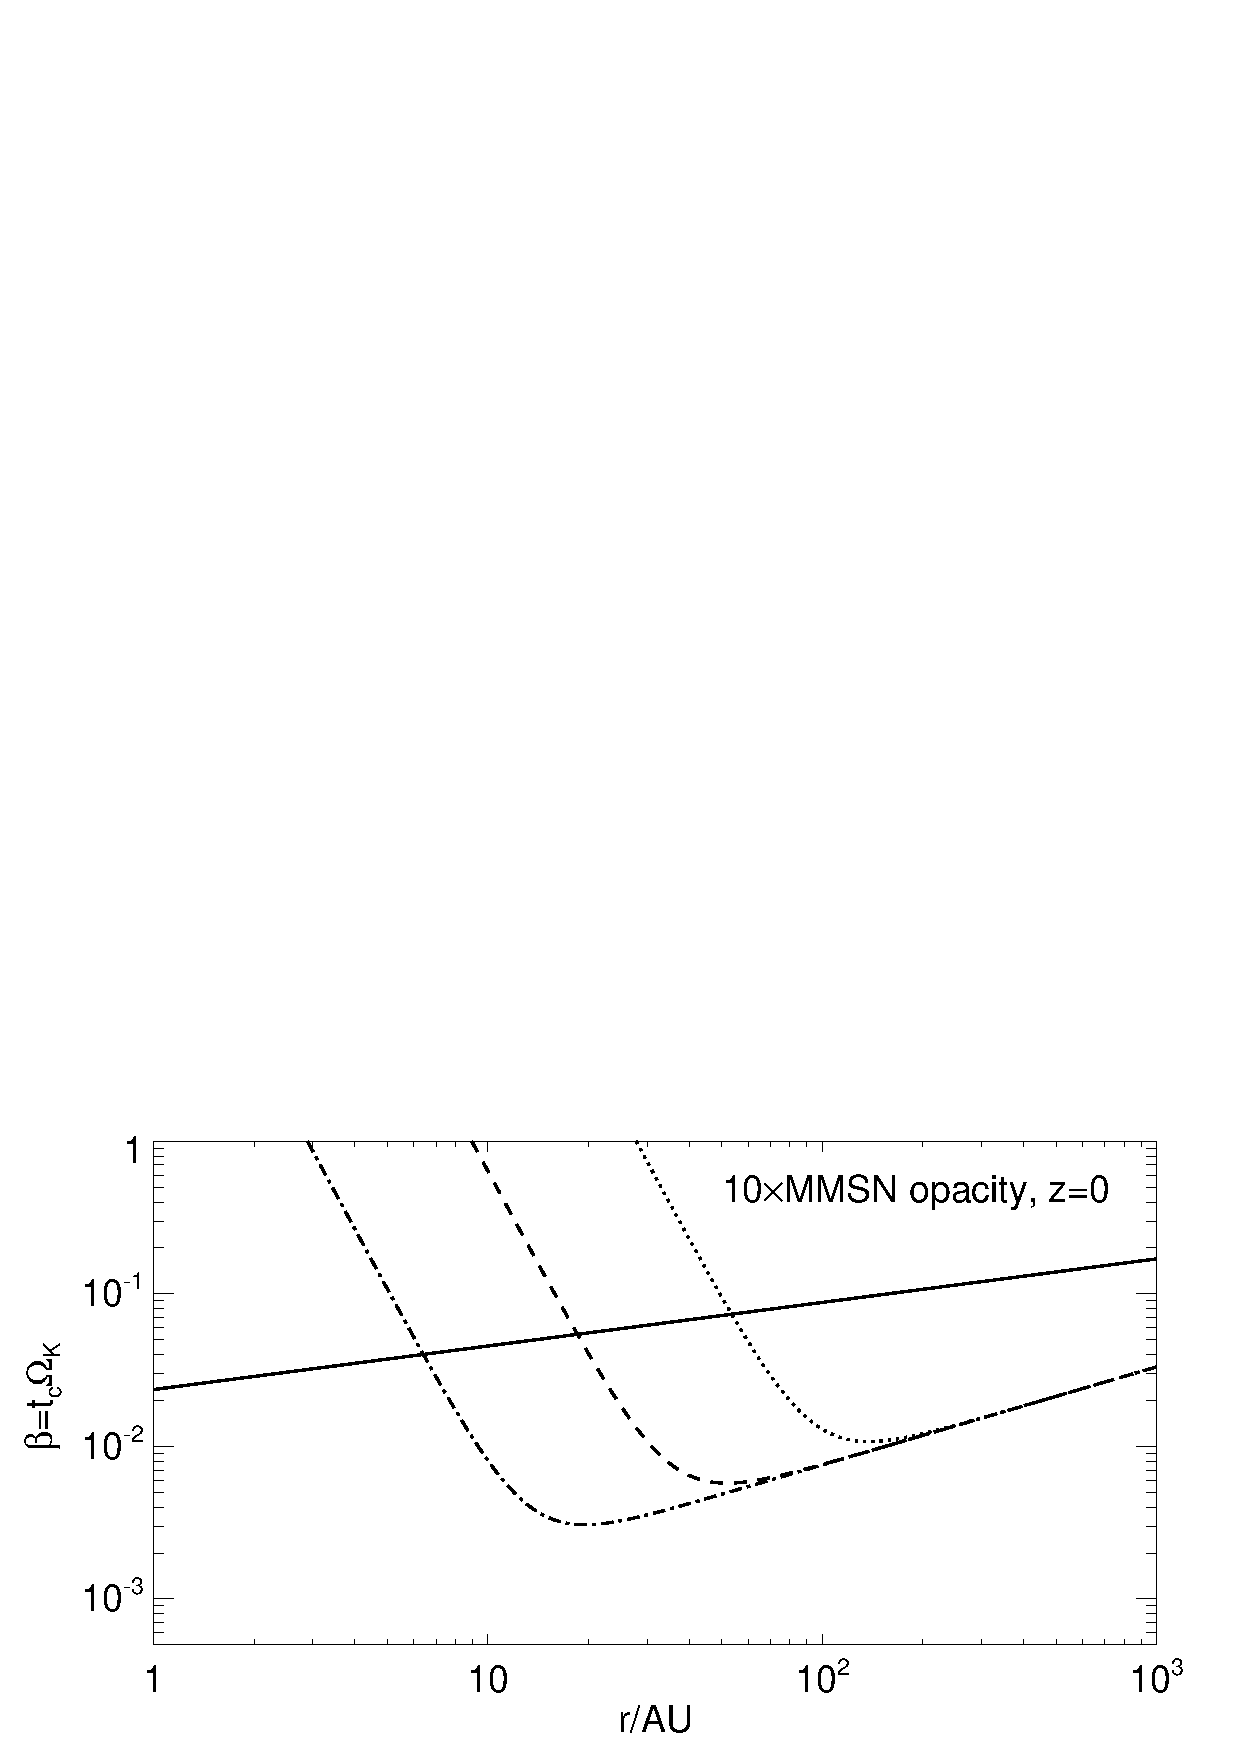
\includegraphics[scale=.47,clip=true,trim=0cm 0cm 0cm
  1cm]{figures/bcrit_mmsn_kap10_z0}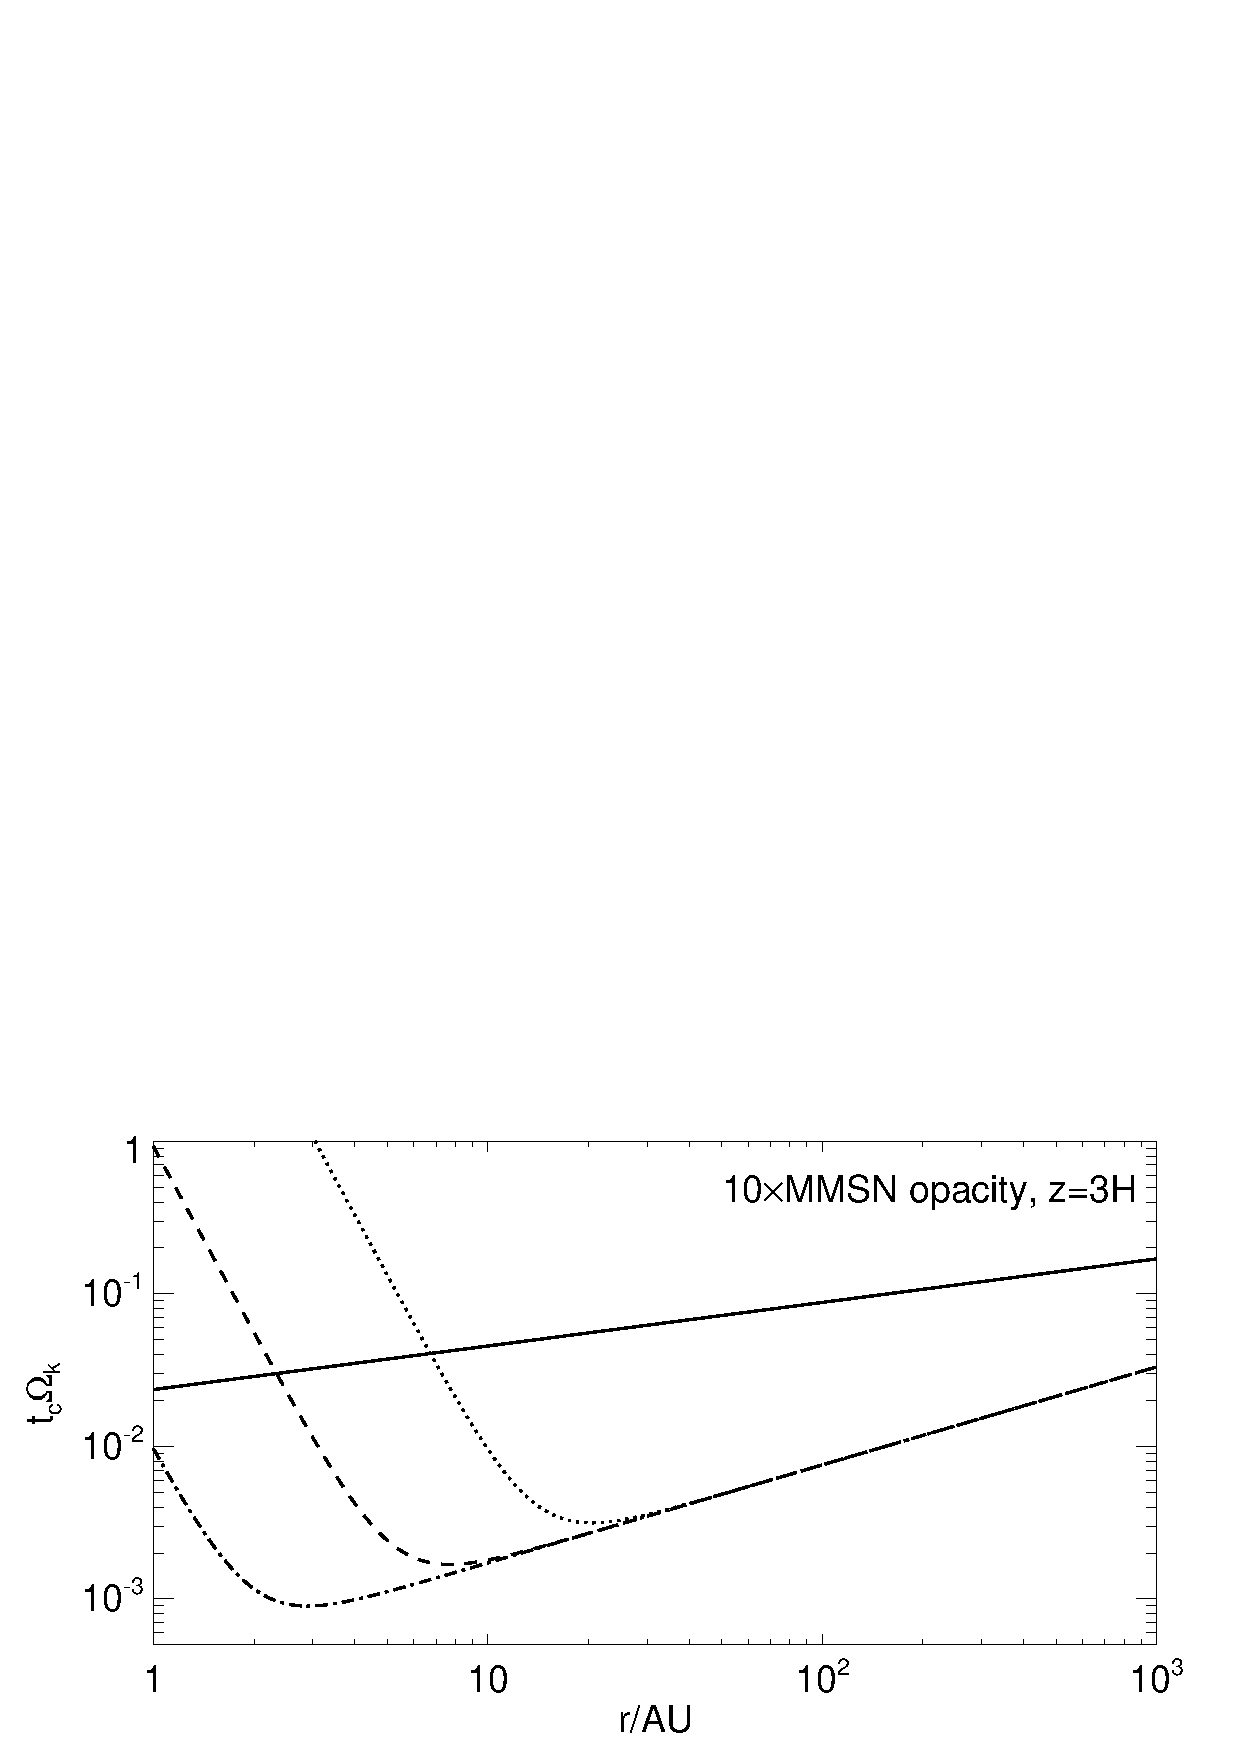
\includegraphics[scale=.47,clip=true,trim=2.5cm 0cm 0cm
  1cm]{figures/bcrit_mmsn_kap10_z3} 
  \caption{Dimensionless thermal relaxation timescales $\beta$,
    evaluated at the midplane (left) and at $z=3H$ (right) in the
    fiducial PPD. Eq. \ref{beta_mmsn_simp} is plotted  
    for three values of the 
    perturbation radial wavenumber: $\khat=1$ (dotted), $\khat=10$
    (dashed) and $\khat=100$ (dashed-dot), for three values of the
    opacity relative to the MMSN: $\hat{\kappa}_d=0.1$ (top),
    $\hat{\kappa}_d=1$ (middle) and $\hat{\kappa}_d=10$ (bottom).  
    The solid line is the 
    critical thermal relaxation timescale $\beta_\mathrm{crit}$.  
    \label{mmsn_bcrit_bcool}}   
\end{figure*}  

In Fig. \ref{mmsn_bcrit_bcool}, we compare $\beta$ to
$\beta_\mathrm{crit}$ across a range of disk radii for different
heights, opacity values and wavenumbers. 
For optically thin cooling in the outer disk, curves for different
wavenumbers overlap, as expected from Eq.\ \ref{beta_mmsn_simp}. 
Since the (optically thin) slope of $\beta$ is slightly steeper than
for $\beta_\mathrm{crit}$, VSI growth can be suppressed at large radii
(for the chosen opacity law).  This effect is seen for $\hat{\kappa}_d
= 1$ in the central panels of Fig.\ \ref{mmsn_bcrit_bcool}, where VSI
is damped outside $\sim 150$ AU. 

We find that the most important factor for VSI growth is the opacity.
With a smaller opacity, $\hat{\kappa}_d = 0.1$, growth is suppressed
at all radii, as shown in the top panels of Fig.\
\ref{mmsn_bcrit_bcool}.  Since optically thin cooling is too slow in
this case, optically thick cooling --- above the floor set by optically
thin cooling --- is also too slow.   

Larger opacities make optically thin cooling much faster than $\beta_\mathrm{crit}$, as shown in the top panels of Fig.\ \ref{mmsn_bcrit_bcool}.  However with larger opacities, optically thick cooling affects larger disk radii, slowing the cooling.  Remarkably, the adopted MMSN value of opacity hits the a sweet spot where optically thin cooling is fast enough, yet slower optically thick can be restricted to inner disk radii.

At smaller disk radii,  Fig. \ref{mmsn_bcrit_bcool} shows the hallmark of diffusive cooling, that larger wavenumbers can cool faster, but not below the floor set by optically thin cooling.  Optically thick cooling times also rise sharply toward smaller radii (as $\beta \propto r^{-57/14}$) due to high densities and short orbital times.  This effect suppresses VSI growth at small radii, but with a strong wavenumber dependence. 



%for $r_\mathrm{AU}\in[1,100]$, as well as for different
%opacity scales. Notice that $\beta$ increases for either large or
%small radii. For sufficiently large $r$, disturbances are generally
%in the optically-thin cooling regime, characterized graphically by the
%over-lapping curves. 
%%, where $\beta$ is independent of
%%$z$ and the perturbation lengthscale $\khat$.
%In this case, we may
%directly compare $\beta$ to $\beta_\mathrm{crit}$ and infer that the
%VSI can operate at 10s of AU in the fiducial MMSN disk (with
%$\hat{\kappa}_d=1$).  However, at small radii, $\beta$ depends on both
%$z$ and $\khat$, as the disturbance enters the optically-thick limit
%at the midplane. This regime is characterized by the distinct curves for each
%$\khat$ toward decreasing $r$.  
%  
%%\emph{a better organized discussion might end on this point.  Might not be easy to rearrange to do this, but it would ideal to have the seamless flow to what you do next.}
% 
%Next consider the effect of the opacity scale $\hat{\kappa}_d$. The previous section
%(see also Eq. \ref{beta_mmsn_simp}) indicates that increasing $\hat{\kappa}_d$
%increases (decreases) the cooling time in the optically thick (thin)
%limits. The overall effect of  increasing (decreasing) the opacity
%scale by an order of magnitude is illustrated in the lower (upper)
%panels of Fig. \ref{mmsn_bcrit_bcool}. 
%
%For increasing opacity, $\hat{\kappa}_d=1\to 10$,  a comparison
%between the middle and lower panels shows that the optically-thick
%regions shift outward; while the
%optically-thin regions have lowered cooling times. Thus, instability
%is expected to be restricted to larger radii. 
%
%For decreasing opacity, $\hat{\kappa}_d=1\to 0.1$,  the
%optically-thick regions shift inwards; while cooling times in the
%optically-thin limit are increased. In fact, the latter effect is
%significant enough to raise $\beta > \beta_\mathrm{crit}$ over all
%radii, and even away from the midplane. This is expected to stabilize
%the disk against the VSI.  

\begin{figure}
  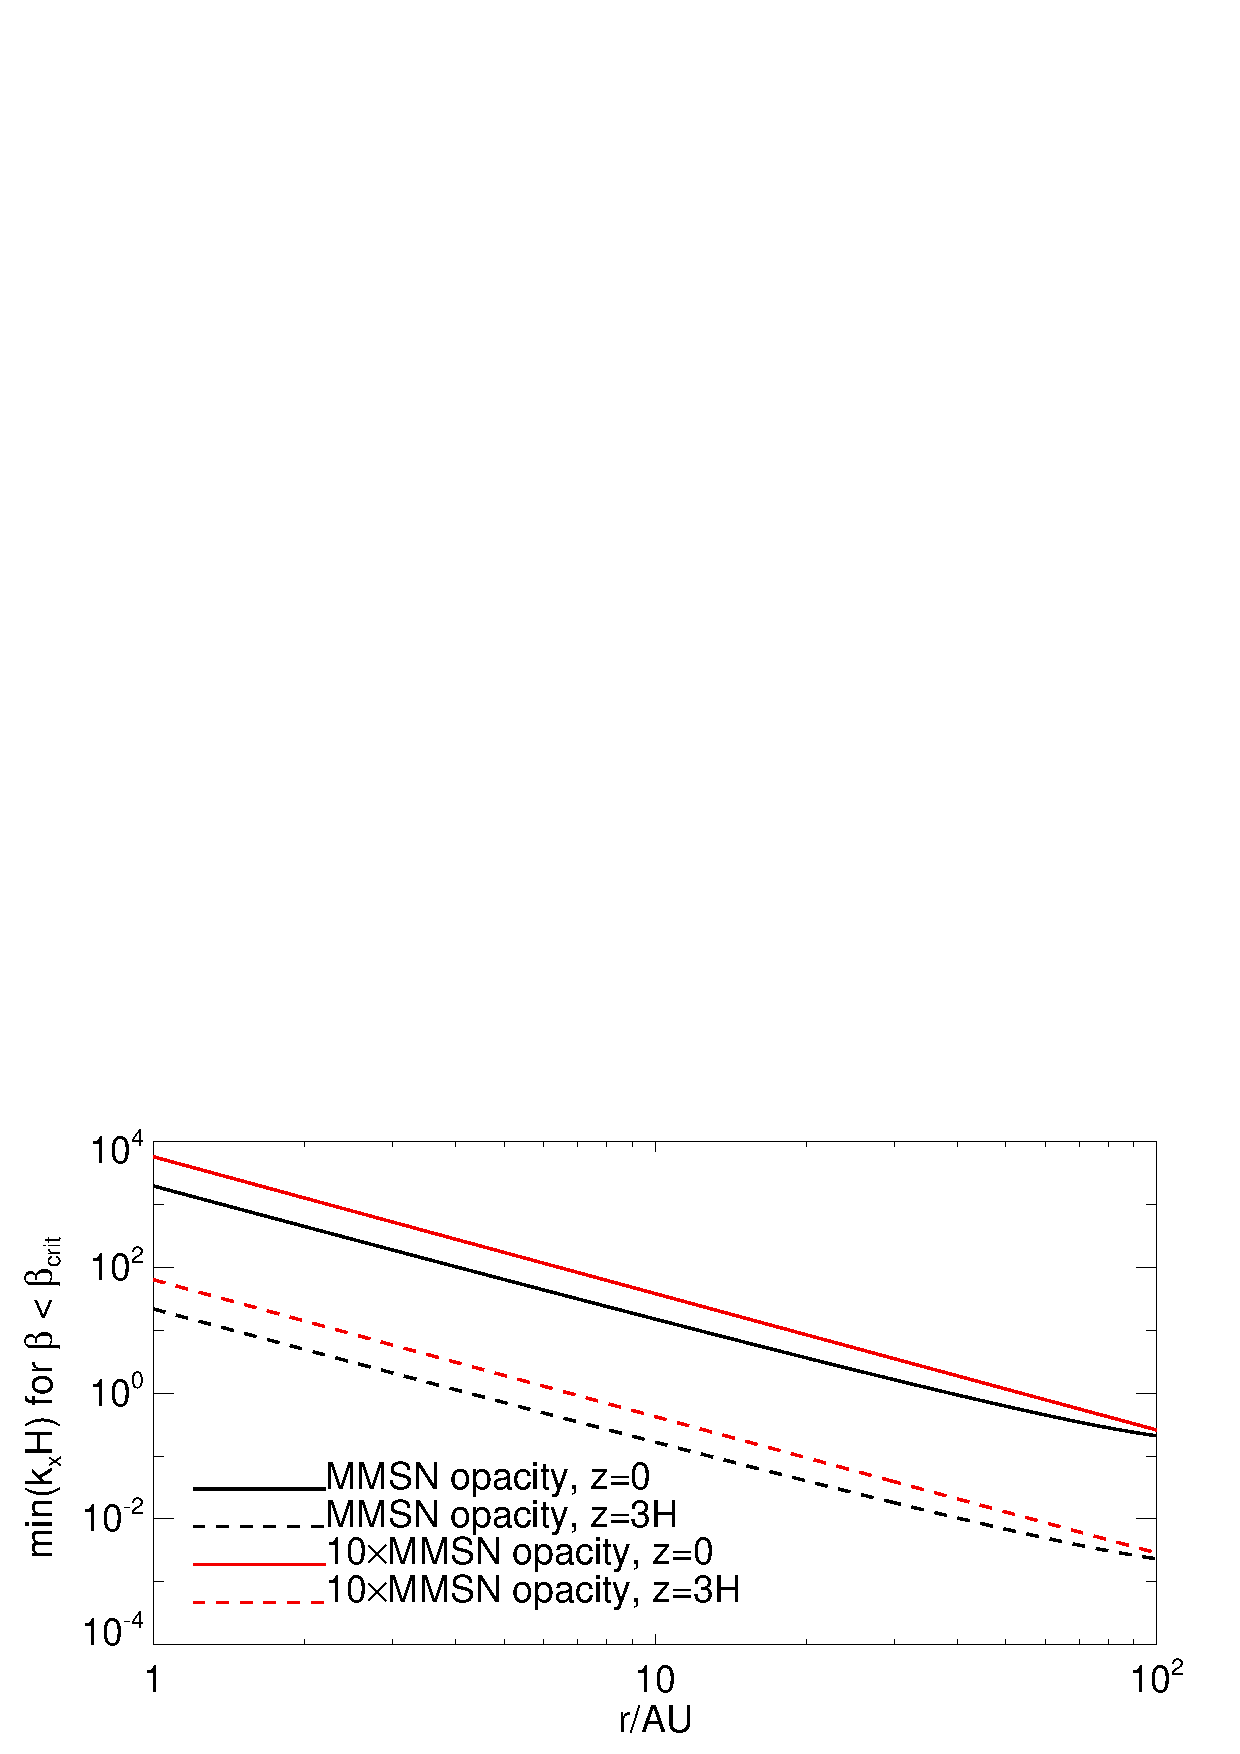
\includegraphics[width=\linewidth]{figures/bcrit_mink} 
  \caption{The minimum perturbation wavenumber $\khat$ in
    the MMSN such that the associated dimensionless thermal
    relaxation time $\beta$ at $z=0$ (solid) and $z=3H$ (dashed) is
    less than the critical timescale $\beta_\mathrm{crit}$.   
    \label{mmsn_bcrit_bcool_mink}}   
\end{figure}  

Fig. \ref{mmsn_bcrit_bcool_mink} highlights this wavenumber dependence by plotting
the wavenumbers for which $\beta = \beta_\mathrm{crit}$.  Above the solid curves (i.e.\ for larger wavenumbers), $\beta <  \beta_\mathrm{crit}$ at all disk heights, implying linear VSI growth.  Below the dashed curves, VSI growth is strongly suppressed since $\beta >  \beta_\mathrm{crit}$ for all $|z| > 3H$.  Between the solid and dashed curves some growth is possible, but only fairly close to the solid curve (according to \S\ref{vsi_mmsn_grow}).  Thus linear growth of the VSI near 1 AU is only possible if $k_x \gtrsim 10^3/H$.  As argued elsewhere, we doubt that such small-scale disturbances will drive significant turbulence or transport.

We thus doubt that the VSI is significant at 1 AU in MMSN-like PPDs, for any opacity.  At higher opacities, the required wavenumbers become shorter and even more problematic, as shown by the red curves in Fig. \ref{mmsn_bcrit_bcool_mink}.  At lower opacties, even optically thin cooling (the fastest possible) is too slow, as discussed above. 

\emph{Big question, do we need to include disk mass as another parameter to vary.  Or not in this study.  Has been included in SK14.}

%In the disk
% atmosphere where $\beta$ is small, surface modes may develop, 
% but they are not well-defined in vertically isothermal disk models
% with an imposed boundary, and they also require large $\khat$. 


\subsection{VSI growth in the MMSN}\label{vsi_mmsn_grow}
We now consider the growth of the VSI in a MMSN disk model.  The linear analysis is similar to 
\S\ref{numerical} but with different disk parameters and with the self-consistent cooling times of 
Eq. \ref{beta_mmsn_simp}. 

We consider the growth timescales of the fundamental mode for a range of
wavenumbers and disk radii. We focus on the fundamental, i.e. lowest order vertical, mode 
because it is the fastest growing mode except for some surface modes at high 
wavenumbers.   We neglect these surface modes for reasons disucssed in \S\ref{numerical} and \S\ref{caveats_visc}.

%  which are 
% boundary-dependent. 
% Disturbances with large $\khat$ are also more likely subject to viscous 
% decay, as discussed above. 
 %\\
%\emph{above sentence too long and complex, could e.g.\ split off that surface modes are neglected and why.}
%However, surface modes are dependent on
%boundary conditions in a vertically isothermal disk \citep{barker15},  
%and 

Fig. \ref{mmsn_overall} shows that in the MMSN, the VSI  is active from $r_\mathrm{AU}\sim 5$ to $r_\mathrm{AU}\sim
50$ with growth timescales $\sim 30$---40 orbits.  A small radius cufoff exists, inside of which growth is strongly suppressed.  The cutoff occurs at smaller radii for larger wavenumbers, as expected from Fig.\ \ref{mmsn_bcrit_bcool_mink}.  Growth at smaller disk radii is possible for yet larger wavenumbers, yet we remain skeptical about the non-linear viability of such short modes.

The growth times rise gradually as $r$ increases towards 100 AU in Fig. \ref{mmsn_overall}.  This trend is expected as the outer radius cutoff at $\sim 200$AU (from Fig.\ \ref{mmsn_bcrit_bcool}) is approached.


%
%The fact that we can obtain the VSI in the despite $\beta >
%\beta_\mathrm{crit}$ near the midplane (e.g. $\khat = 30$ at
%$r_\mathrm{AU} =5$, see Fig. \ref{beta_compare}) suggests  that the instability
%can operate provided $\beta < \beta_\mathrm{crit}$ for a sufficiently large
%fraction of the vertical domain. However, the normalized growth times
%become much longer. For example, for $\khat=30$ we find
%$t_\mathrm{grow}\sim 40$ orbits at $r_\mathrm{AU}=50$, but $t_\mathrm{grow}\sim
%400$ orbits at $r_\mathrm{AU}=5$ (and rapidly increases to $> 10^3$ orbits for
%smaller $r$). Thus, introducing an optically-thick midplane 
%significantly reduces the efficiency of the VSI despite $\beta <
%\beta_\mathrm{crit}$ away from the midplane. 


%We thus find Fig. \ref{mmsn_overall} to be roughly consistent with
%comparing the midplane thermal relaxation timescales to the critical
%thermal timescale. For example, 
%Fig. \ref{mmsn_bcrit_bcool} show that $\beta(z=0,\khat=10) \gtrsim
%\beta_\mathrm{crit}$ for $r_\mathrm{AU}\lesssim 10$ in the MMSN (left middle
%panel); and Fig. \ref{mmsn_overall} 
%show that modes with $\khat=10$ are stabilized for $r_\mathrm{AU}\lesssim 8$ (where
%$t_\mathrm{grow}\to\infty$). 

\emph{I don't understand the specific comparison being made here, especially since N13 is for vert.\ constant beta.  Maybe remind me of which specific result/figure.  I would think the more relevant comparison is to SK14 (either here or in discussion).}
 Our numerical results suggest the VSI
is efficient at radii of few tens of AU in the MMSN, consistent with
estimates made by \citetalias{nelson13}. 

\begin{figure}
  \includegraphics[width=\linewidth]{figures/eigen_compare_grow.ps}
  \caption{VSI growth times ($t_{\rm grow} = 1/\sigma$) in orbital units ($P_\mathrm{orb} = 2\pi/\OmK$) for
    the reference MMSN disk model with self-consistent dust cooling. 
    \label{mmsn_overall}}    
\end{figure}
